% This file was created with tikzplotlib v0.9.12.
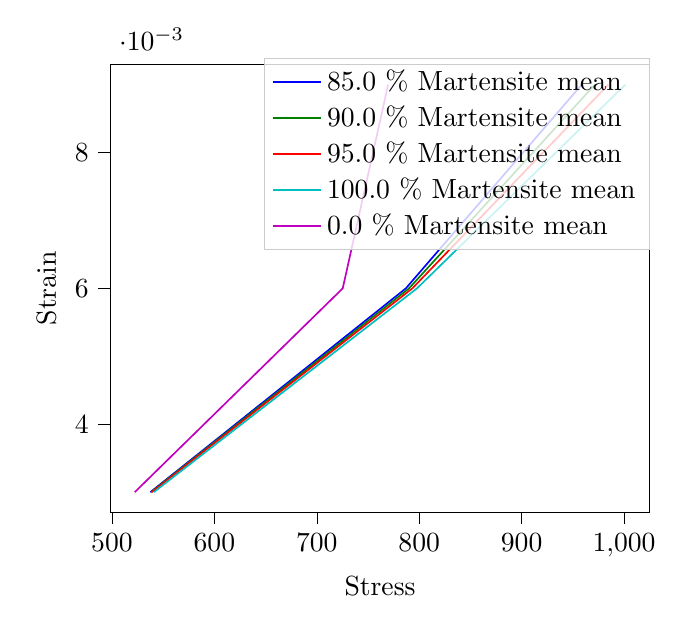
\begin{tikzpicture}

\definecolor{color0}{rgb}{0,0.75,0.75}
\definecolor{color1}{rgb}{0.75,0,0.75}

\begin{axis}[
legend cell align={left},
legend style={
  fill opacity=0.8,
  draw opacity=1,
  text opacity=1,
  at={(1,0.8)},
  anchor=east,
  draw=white!80!black
},
tick align=outside,
tick pos=left,
x grid style={white!69.0196078431373!black},
xlabel={Stress},
xmin=498.28667, xmax=1025.22473,
xtick style={color=black},
y grid style={white!69.0196078431373!black},
ylabel={Strain},
ymin=0.0027, ymax=0.0093,
ytick style={color=black}
]
\addplot [semithick, blue]
table {%
537.5012 0.003
786.94065 0.006
958.72575 0.009
};
\addlegendentry{85.0 \% Martensite mean}
\addplot [semithick, green!50!black]
table {%
538.18685 0.003
790.0433 0.006
971.5101 0.009
};
\addlegendentry{90.0 \% Martensite mean}
\addplot [semithick, red]
table {%
538.8505 0.003
793.2877 0.006
984.7113 0.009
};
\addlegendentry{95.0 \% Martensite mean}
\addplot [semithick, color0]
table {%
540.8715 0.003
797.823 0.006
1001.273 0.009
};
\addlegendentry{100.0 \% Martensite mean}
\addplot [semithick, color1]
table {%
522.2384 0.003
725.30785 0.006
769.6578 0.009
};
\addlegendentry{0.0 \% Martensite mean}
\end{axis}

\end{tikzpicture}
